% !TeX root = ..\essay.tex

\section{Evaluation}
\label{ch:evaluation}

\subsection{evaluation setting}
To evaluate the summaries they were manually annotated.
Each summary has been annotated by at least four raters with the following criteria:
\begin{table}[H]
	\begin{tabularx}{\textwidth}{l|X} \toprule
		criteria & description \\ \midrule
		Grammaticality      & \\
		Non-Redundancy      & \\
		Referential Clarity & \\
		Focus               & \\
		Structure           & \\
		Coherence           & \\
		Readability         & \\
		Information Content & \\
		Spelling            & \\
		Length              & \\
		Overall Quality     & \\ \bottomrule
	\end{tabularx}
	\caption{evaluation criteria}
	\label{tab:evacriteria}
\end{table}

The score for each criteria was set with the help of a five-point Likert scale with the following scales:

\begin{enumerate}
	\item very poor
	\item poor
	\item barely acceptable
	\item good
	\item very good
\end{enumerate}

For each criteria the opportunity to give an estimation in weighting and confidence would be expected, too.
These further possibilities to rate a summary are also realized with a five-point Likert scale.
In table~\ref{tab:evalikert} the scales for Weight and Confidence are shown:

\begin{table}[H]
	\begin{tabularx}{\textwidth}{l|XX} \toprule
		Scale & Weight & Confidence \\ \midrule
		1 & completely unimportant & very low \\
		2 & unimported & low \\
		3 & indifferent & half sure \\
		4 & important & high \\
		5 & absplutely important & very high \\ \bottomrule    
	\end{tabularx}
	\caption{Likert scale for Weight and Confidence}
	\label{tab:evalikert}
\end{table}

The annotators had also the opportunity to comment each criteria for each summary with free text.

\subsection{JSD}

\begin{figure}[H]
	\centering
	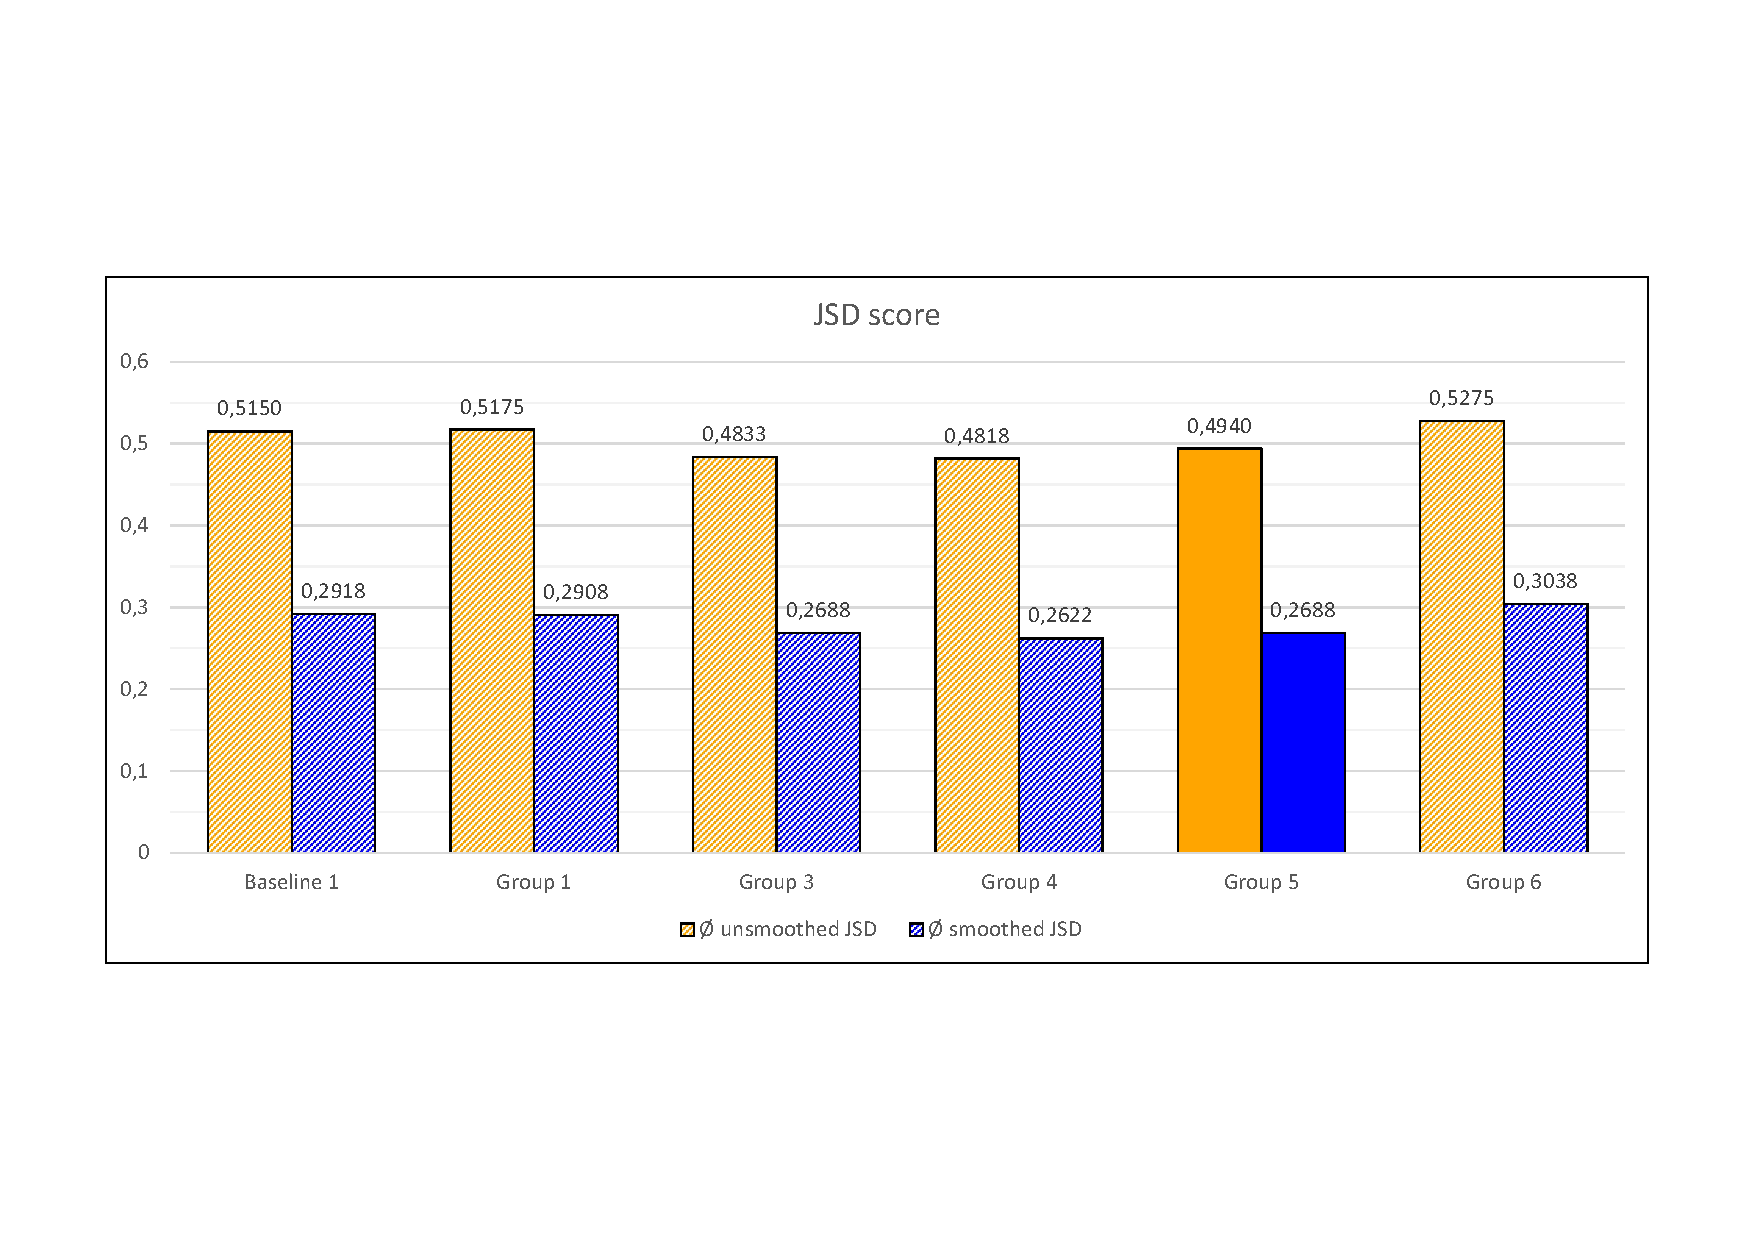
\includegraphics[trim= 0 150 0 150,width=\textwidth]{img/jsd.pdf}
	\caption{JSD values}
	\label{fig:jsd}
\end{figure}


\subsection{Scores per Criteria}

\begin{figure}[H]
	\centering
	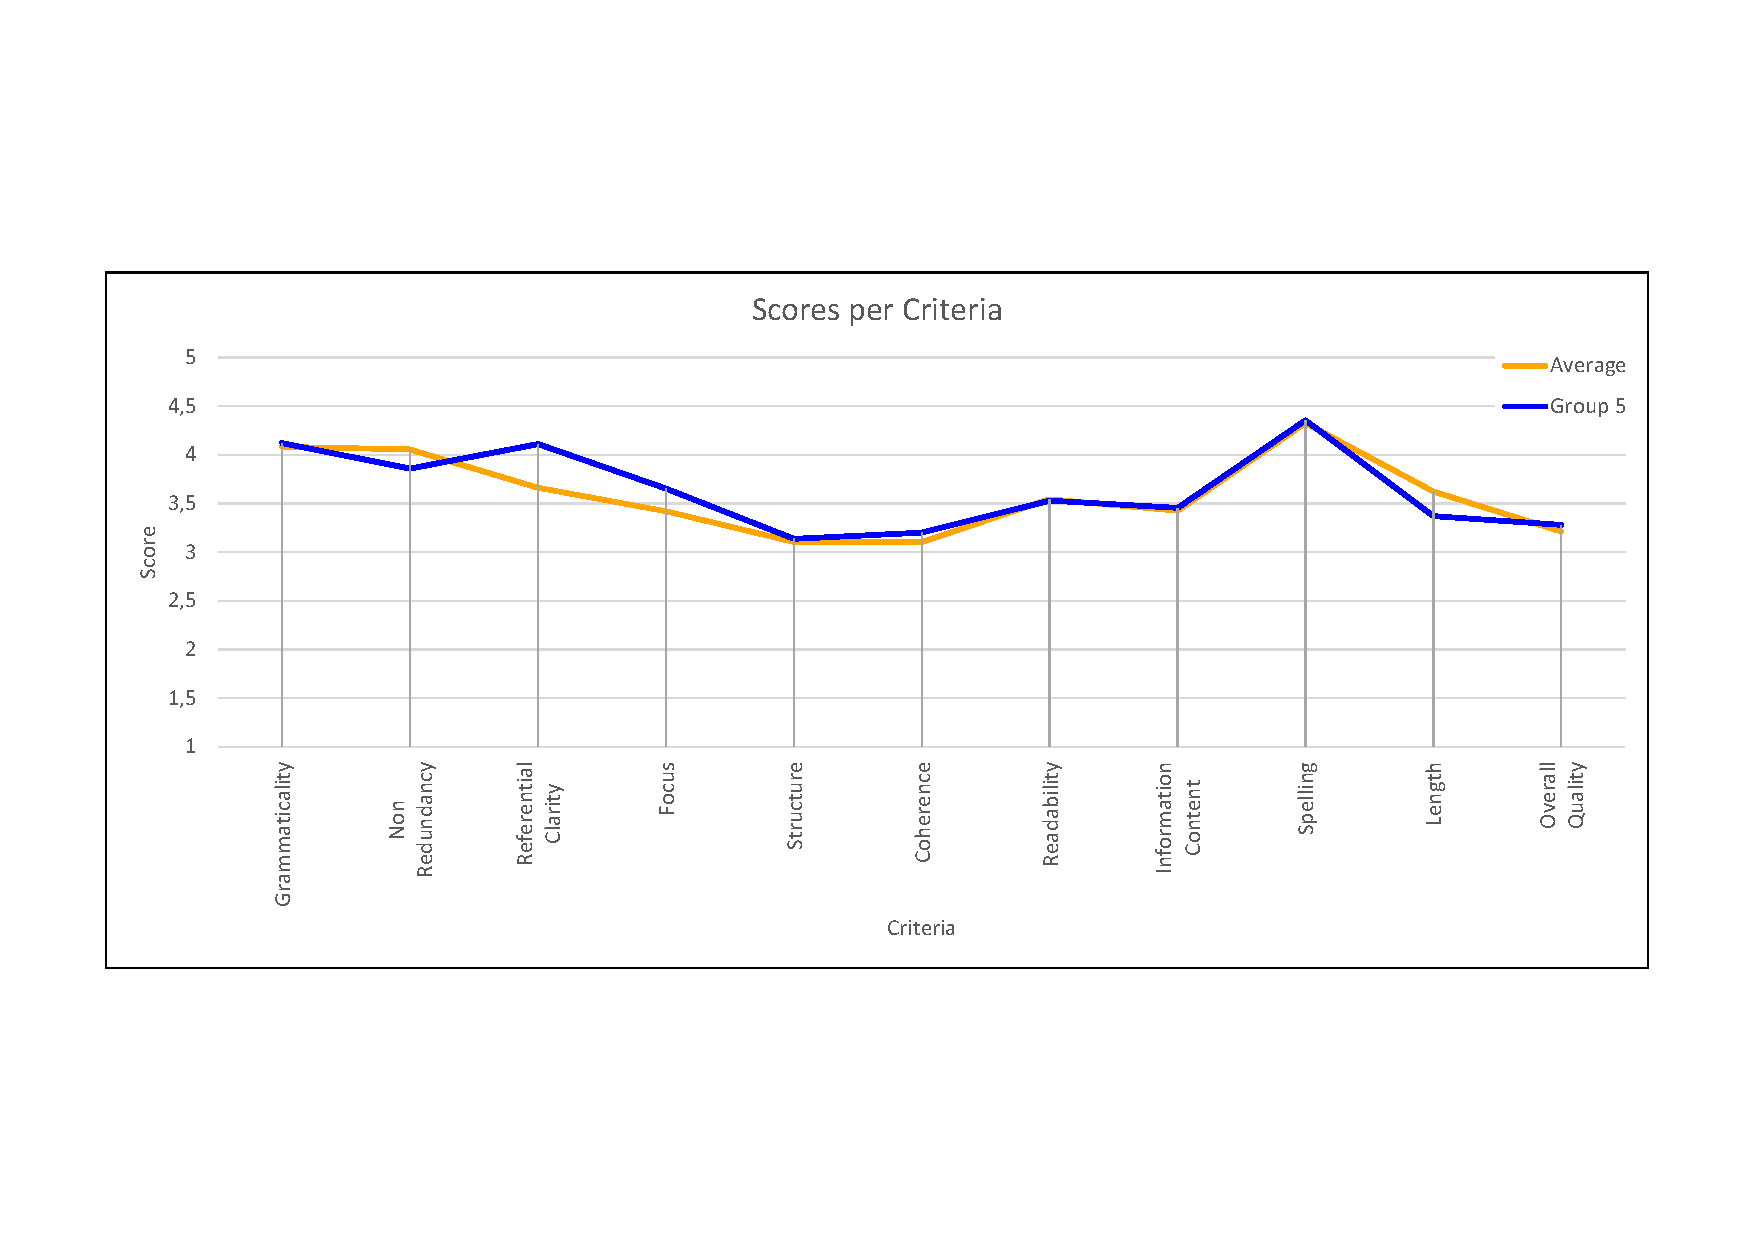
\includegraphics[trim= 0 150 0 150,width=\textwidth]{img/scores_per_criteria.pdf}
	\caption{scores per criteria}
	\label{fig:spc}
\end{figure}

\subsection{why so good / bad}
free text analysis per criteria


\subsection{box plot}

\begin{figure}[H]
	\centering
	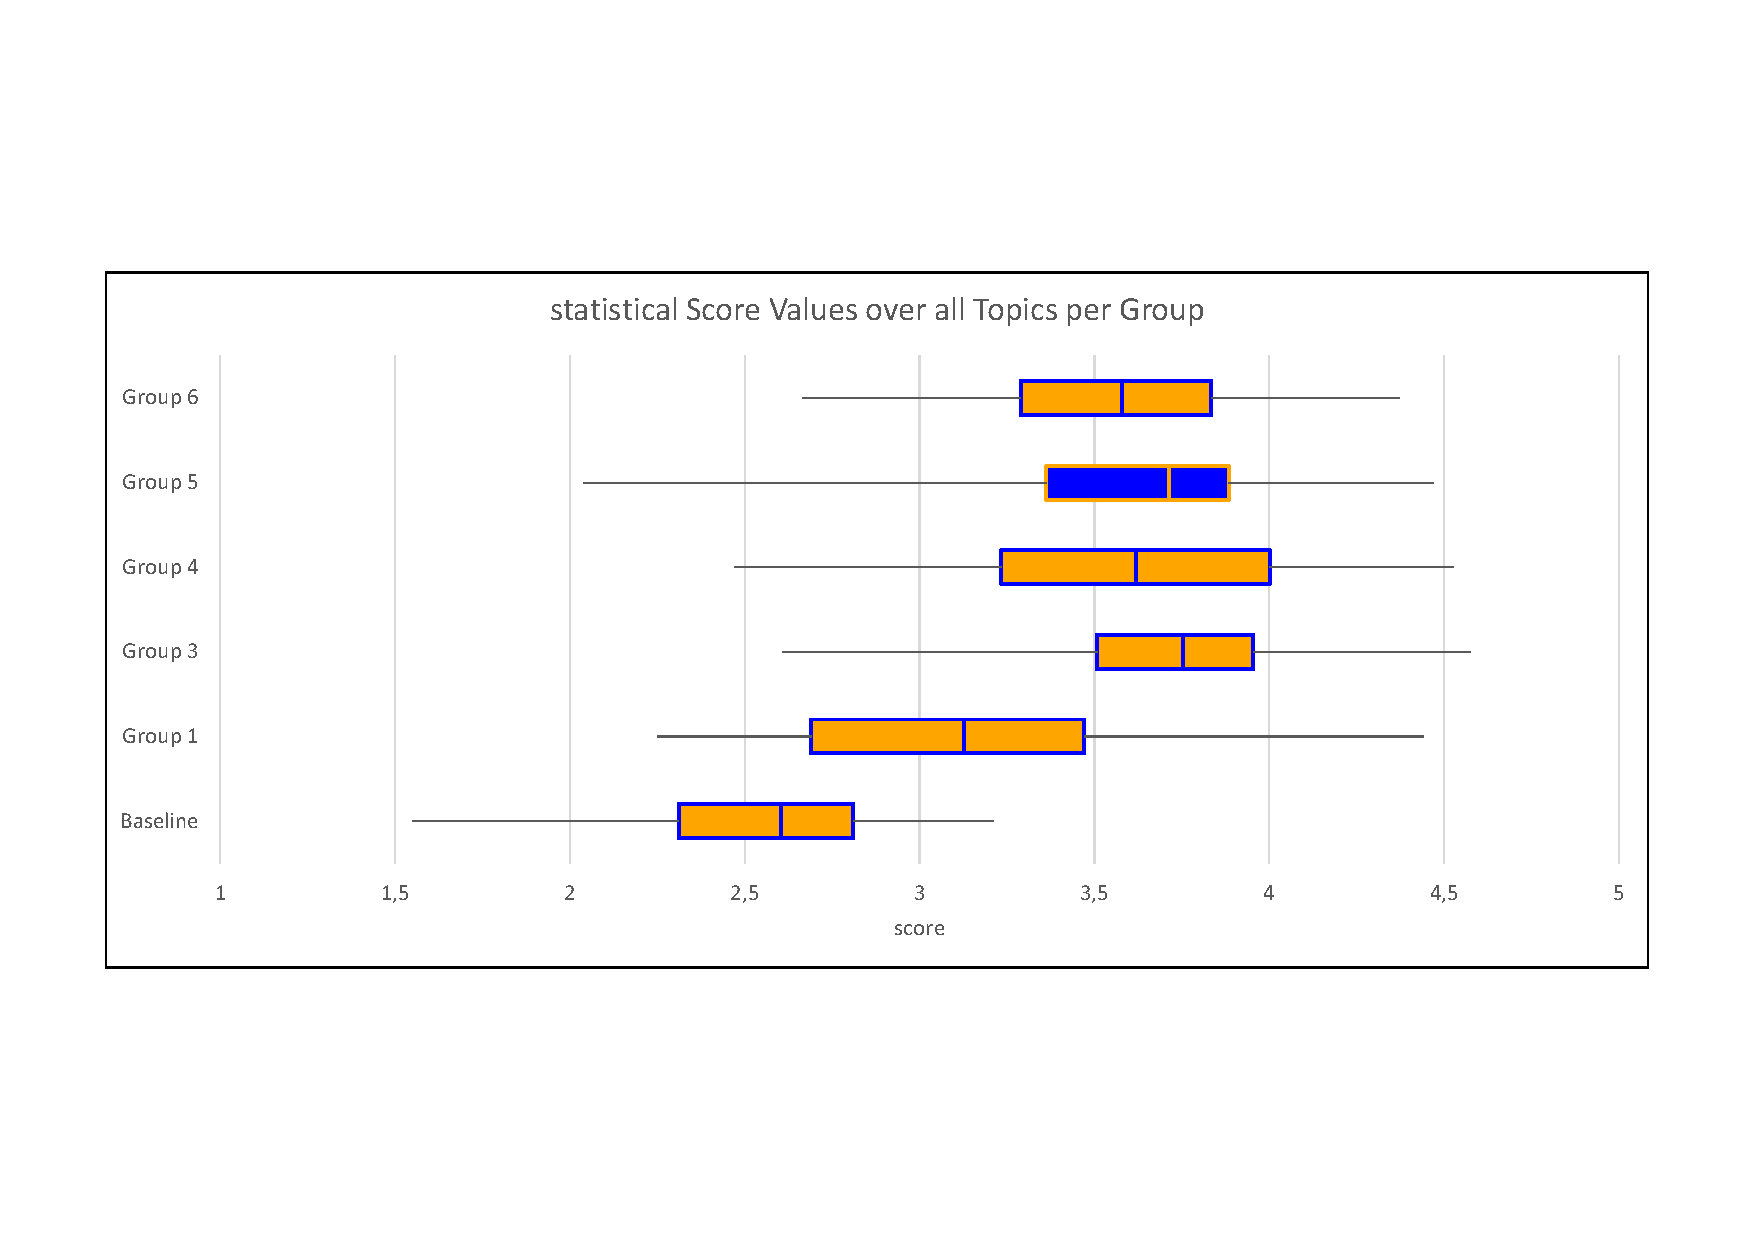
\includegraphics[trim= 0 150 0 150,width=\textwidth]{img/box.pdf}
	\caption{statistical values over all topics per group}
	\label{fig:svg}
\end{figure}


\subsection{Score Calculation with all scales}

\begin{figure}[H]
	\centering
	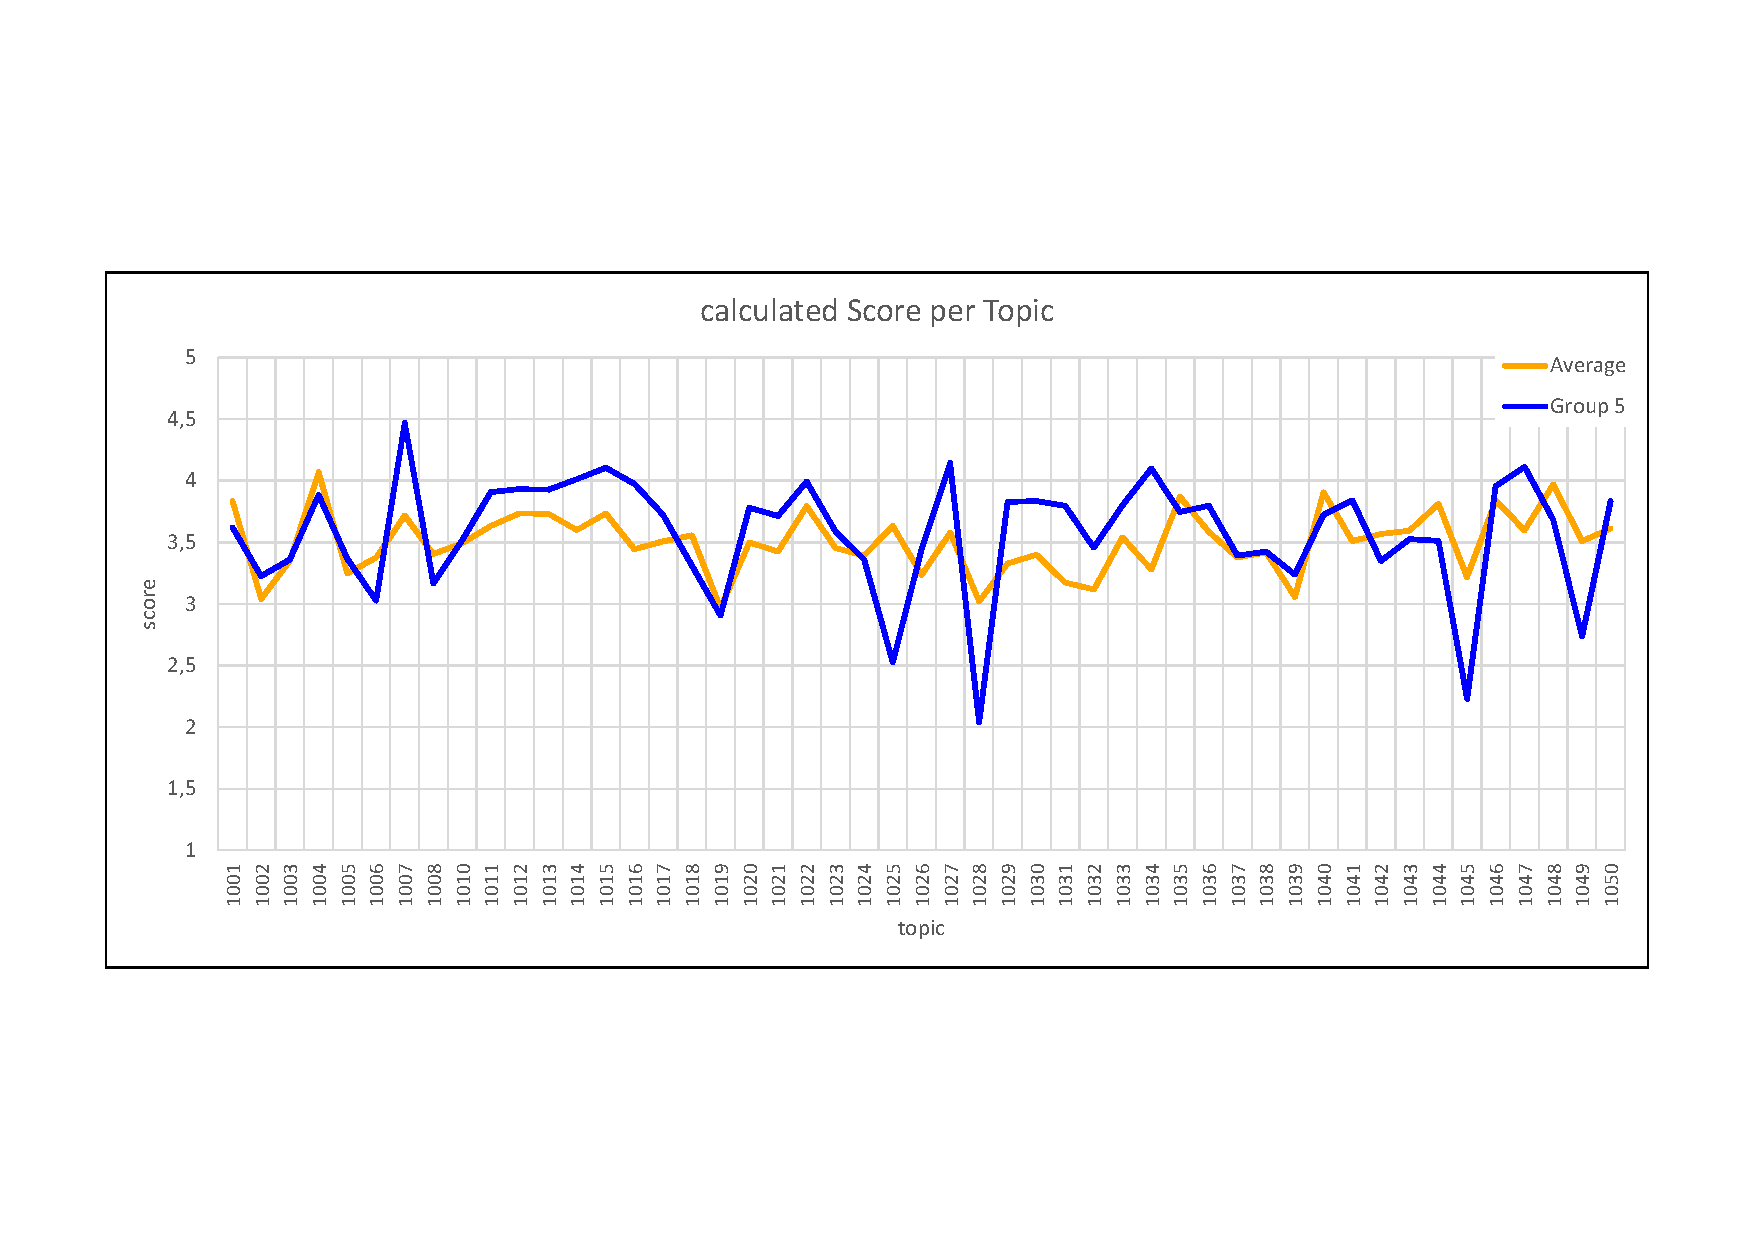
\includegraphics[trim= 0 150 0 150,width=\textwidth]{img/score_per_topic.pdf}
	\caption{scores per topic}
	\label{fig:spt}
\end{figure}


\subsection{calculated score per topic - sorted}

\begin{figure}[H]
	\centering
	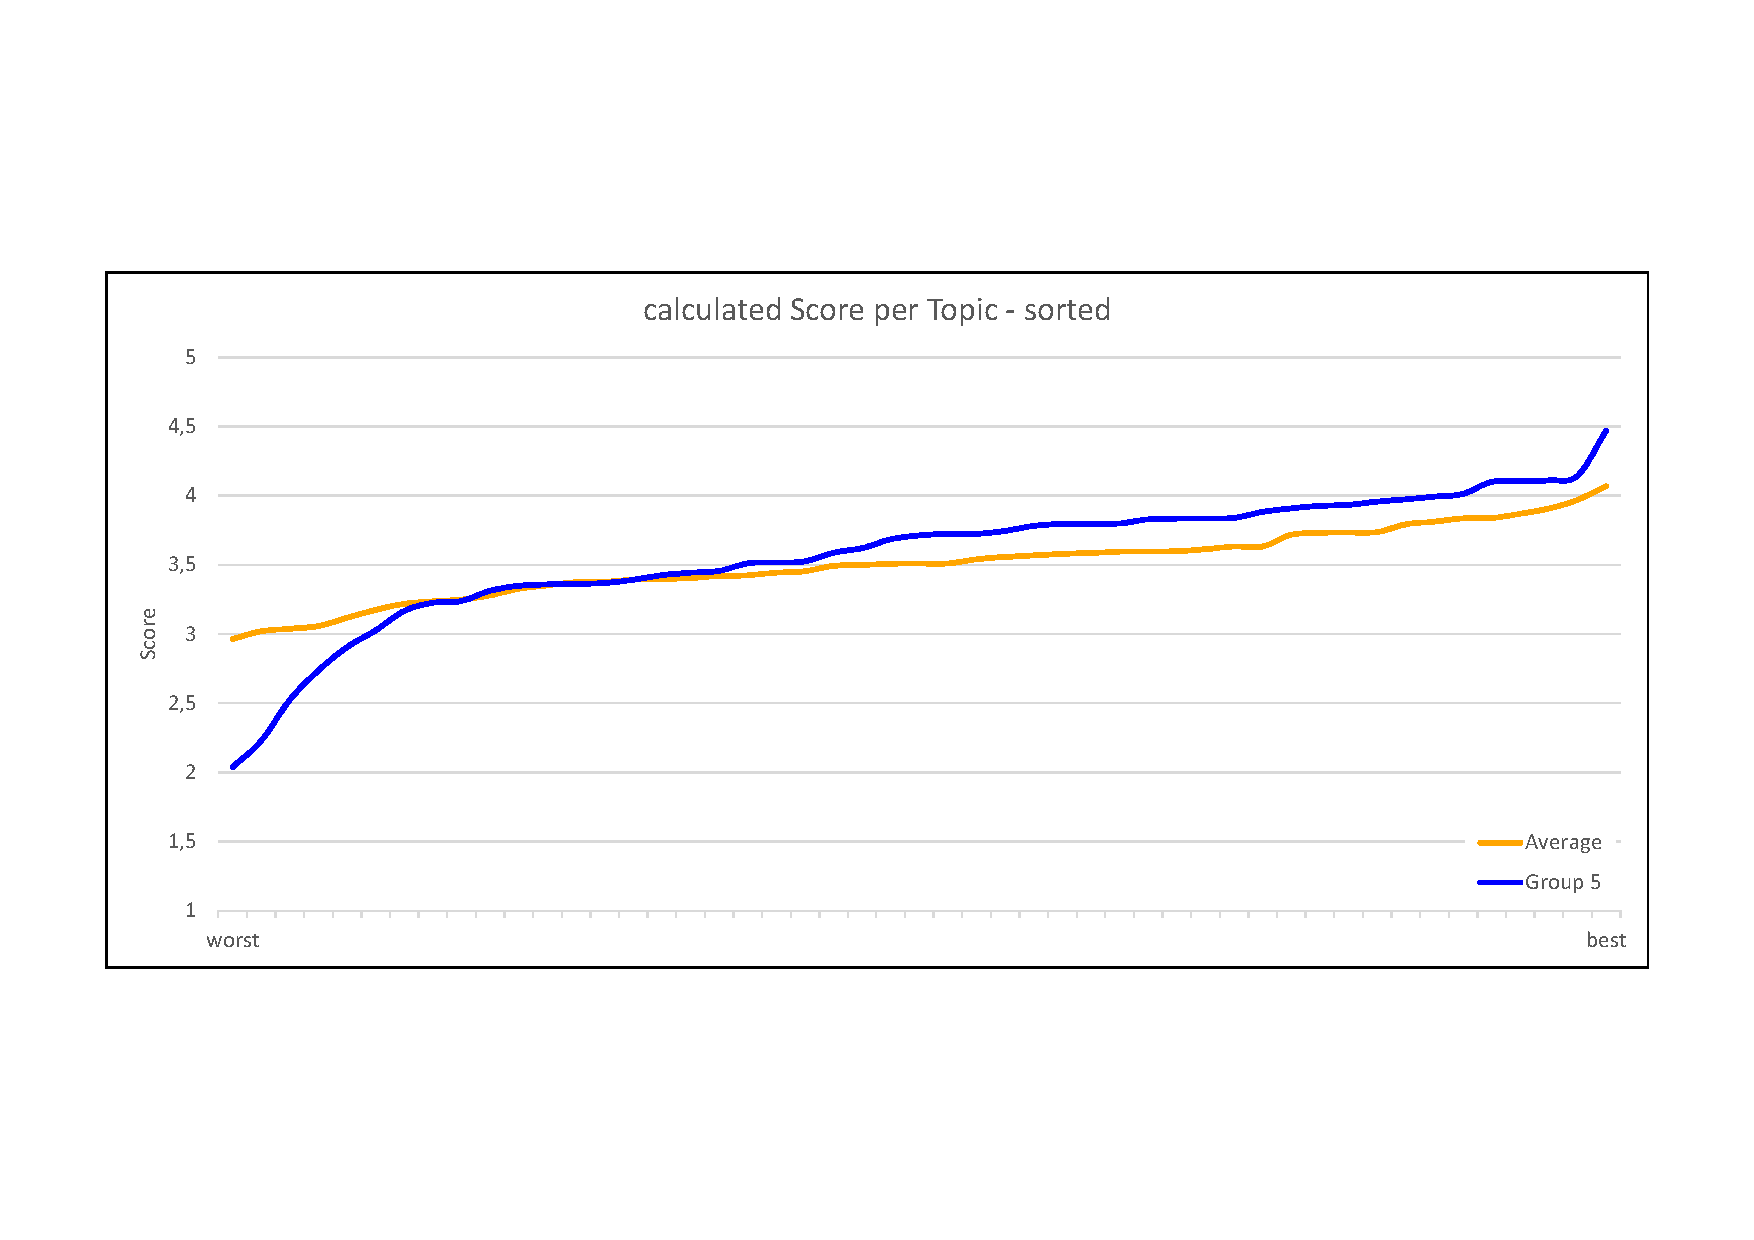
\includegraphics[trim= 0 150 0 150,width=\textwidth]{img/score_per_topic_sorted.pdf}
	\caption{scores per topic sorted ascending}
	\label{fig:spts}
\end{figure}

\subsection{best and worst}